\documentclass[11pt]{article}

\usepackage[margin=1in]{geometry}
\usepackage[T1]{fontenc}
\usepackage[utf8]{inputenc}
\usepackage{lmodern}
\usepackage{microtype}
\usepackage{amsmath,amssymb,mathtools}
\usepackage{booktabs,tabularx,array}
\usepackage{enumitem}
\usepackage{tikz}
\usetikzlibrary{arrows.meta,positioning,fit}
\usepackage[hidelinks]{hyperref}
\usepackage{xcolor}
\usepackage{fancyhdr}
\usepackage{lastpage}

\definecolor{muted}{gray}{0.35}
\definecolor{rulegray}{gray}{0.78}
\newcommand{\Austurusa}{\textsc{Austurusa}}
\newcommand{\codeid}[1]{\texttt{#1}}
\newcommand{\doop}{\operatorname{do}}
\newcommand{\cmark}{\ensuremath{\checkmark}}

\setlength{\parindent}{0pt}
\setlength{\parskip}{0.65em}
\setlist[itemize]{leftmargin=1.5em,itemsep=0.25em,topsep=0.25em}
\setlist[enumerate]{leftmargin=1.7em,itemsep=0.35em,topsep=0.3em}
\renewcommand{\arraystretch}{1.18}

\pagestyle{fancy}
\fancyhf{}
\fancyhead[L]{\small\color{muted}\Austurusa\quad /\quad \codeid{AP-002}}
\fancyhead[R]{\small\color{muted}Problem statement v0.1}
\fancyfoot[C]{\small\color{muted}\thepage\ / \pageref{LastPage}}
\renewcommand{\headrulewidth}{0.3pt}
\renewcommand{\footrulewidth}{0pt}

\hypersetup{
  pdftitle={AP-002: Adaptive Causal Worlds},
  pdfauthor={Jack Shaquer / Austurusa},
  pdfsubject={Causal inference under uncertain structural priors},
  pdfkeywords={causal inference, causal foundation models, prior shift, uncertainty, structural causal models}
}

\begin{document}

\thispagestyle{empty}
\vspace*{0.7in}

{\large\texttt{AP-002}}\\[0.55em]
{\Huge\bfseries Adaptive Causal Worlds}\\[0.45em]
{\Large Causal inference when the model may be wrong about the kind of world it inhabits}

\vspace{1.2em}
\rule{\textwidth}{0.5pt}
\vspace{1.0em}

{\large\Austurusa}\\
Jack Shaquer\\
Problem statement v0.1\\
18 September 2026\\[0.5em]
{\color{muted}Status: open, active; exploratory; not peer reviewed; no novelty claim made in this note.}

\vfill

\begin{quote}
\large
Most causal models reason inside assumptions about how the world works. AP-002 asks whether a system can first represent uncertainty about \emph{which family of causal assumptions is appropriate}, recognize when its familiar families do not explain the evidence, and seek information that can distinguish between plausible alternatives.
\end{quote}

\vfill
\rule{\textwidth}{0.4pt}
{\small\color{muted}
Austurusa is an independent open-idea organization for difficult problems in science and engineering. Work is separated by status: problem statements are not presented as established results or peer-reviewed publications.
}
\newpage

\section*{Abstract}

Modern causal foundation models can be trained on large collections of simulated structural causal models and then estimate causal effects on new datasets without task-specific retraining. This creates a powerful new paradigm: expensive inference can be amortized into a pretrained model whose behavior reflects a chosen distribution over causal data-generating processes. The same design also creates a fundamental vulnerability. If the real system differs materially from the causal prior used during pretraining, the model can be asked to reason outside the universe it learned.

AP-002 studies this problem at the level of \emph{structural prior uncertainty}. Rather than assuming one causal prior is appropriate, we consider several families of possible causal worlds and ask whether observational evidence can support a calibrated belief over those families before a causal estimate is trusted. The target is not to identify a metaphysically ``true universe'' from finite data. In general that is impossible: different causal models may be observationally equivalent. The target is instead to estimate \emph{compatibility}, preserve ambiguity when the evidence cannot distinguish alternatives, abstain when none of the available families explain the data, and--where interventions are available--select experiments that maximally discriminate between remaining hypotheses.

The initial work is deliberately small-scale. It can be tested with frozen public causal foundation models, synthetic structural causal models, classical estimators, and laptop-scale inference. The first scientific question is whether prior-matched causal models exhibit complementary performance across controlled mechanism families, and whether features of the observed dataset can predict which prior is safer without access to counterfactual ground truth. If this does not survive held-out mechanisms and negative controls, the program fails in its present form.

\section{The question in plain language}

Suppose an intelligent system has learned how cause and effect tend to behave inside a particular family of simulated worlds. In those worlds, relationships may be smooth, noise may be well behaved, hidden confounding may be absent, and interventions may follow a particular structure.

Then the system encounters real data.

The obvious question is:

\begin{center}
\fbox{\parbox{0.88\textwidth}{\centering\bfseries
Before trusting a causal conclusion, can the system determine which kinds of causal worlds remain compatible with what it is observing?
}}
\end{center}

That is different from asking whether a prediction is accurate. Prediction asks what will happen under the observed distribution. Causal inference asks what would happen under an intervention. If the assumed causal structure is wrong, a model may predict observations well while giving a poor answer to an intervention question.

At the highest level, AP-002 asks for the following behavior:

\begin{equation}
\begin{aligned}
\text{observations}
&\;\longrightarrow\;
\text{belief over plausible causal worlds}\\
&\;\longrightarrow\;
\text{causal conclusion, uncertainty, or abstention}.
\end{aligned}
\end{equation}

If the available evidence cannot distinguish worlds, the correct output is not false certainty. It is uncertainty. If an experiment can separate the worlds, the system should be able to identify that experiment.

\section{What ``universes'' and ``worlds'' mean}

The metaphor is useful only if it is made precise.

A \textbf{causal world} is one particular structural causal model (SCM), which we can write schematically as

\begin{equation}
\mathcal{M}=(G,\,f,\,P_{\varepsilon}),
\end{equation}

where $G$ is a directed causal graph, $f$ is the collection of structural mechanisms, and $P_{\varepsilon}$ describes exogenous noise. A world specifies how variables are generated and how the system responds to interventions.

A \textbf{causal universe} in this note is not one SCM. It is a \emph{family or prior distribution} over many possible SCMs:

\begin{equation}
\mathcal{M}\sim\Pi_k.
\end{equation}

One family might heavily favor linear-Gaussian mechanisms. Another might contain nonlinear additive functions. Another might allow heavy-tailed or heteroskedastic noise. Another might allow latent confounding or nonstationary mechanisms.

\begin{figure}[h]
\centering
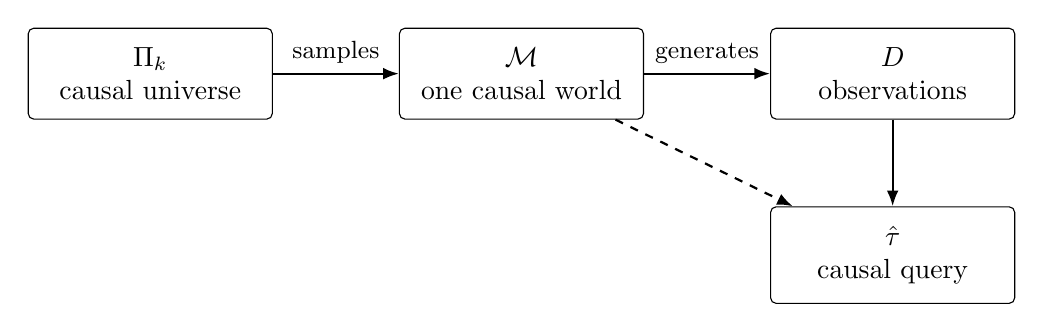
\begin{tikzpicture}[
  node distance=11mm and 16mm,
  box/.style={draw, rounded corners=2pt, inner sep=7pt, align=center, minimum width=31mm},
  arr/.style={-{Latex[length=2mm]}, thick}
]
\node[box] (prior) {$\Pi_k$\\causal universe};
\node[box, right=of prior] (scm) {$\mathcal{M}$\\one causal world};
\node[box, right=of scm] (data) {$D$\\observations};
\node[box, below=of data] (question) {$\hat\tau$\\causal query};
\draw[arr] (prior) -- node[above, font=\small]{samples} (scm);
\draw[arr] (scm) -- node[above, font=\small]{generates} (data);
\draw[arr] (data) -- (question);
\draw[arr, dashed] (scm) -- (question);
\end{tikzpicture}
\caption{A prior or family generates possible causal worlds; a world generates observations and determines the answer to intervention questions.}
\end{figure}

The central concern is therefore not only uncertainty \emph{inside} one assumed family,

\begin{equation}
P(G,\theta\mid D,\Pi_k),
\end{equation}

but uncertainty about the family itself:

\begin{equation}
P(\Pi_k,G,\theta\mid D).
\end{equation}

This is a hierarchical view of causal uncertainty.

\section{Why this question exists now}

Prior-fitted networks (PFNs) make the choice of causal prior especially important. A PFN is trained once on many synthetic tasks sampled from a specified prior and then performs inference on a new dataset in context. CausalPFN applies this idea to treatment-effect estimation and reports competitive causal estimates without per-dataset retraining \cite{balazadeh2025}. CausalFM develops the causal-prior construction more explicitly and trains PFN-based models across back-door, front-door, and instrumental-variable settings \cite{ma2026}.

The attraction is obvious: a difficult inferential workflow can be compressed into a reusable model. But the pretrained model necessarily inherits assumptions from the data-generating distribution used to train it.

CausalPFN already demonstrates a warning sign. Its uncertainty is reported as calibrated in-distribution, while under out-of-distribution data-generating processes it can become severely overconfident; the authors introduce a post-hoc regression-based temperature calibration procedure to repair coverage \cite{balazadeh2025}. This is important prior work and means that simply showing ``OOD causes overconfidence'' is not an AP-002 contribution.

More recently, CausalArena argues that evaluation itself is highly sensitive to the structural causal model family used to generate test environments. It reports substantial ranking shifts across SCM families and highlights pretraining--evaluation overlap as a central issue for causal discovery foundation models \cite{li2026}.

Taken together, these results motivate a stronger question:

\begin{center}
\emph{Can the system reason explicitly about the suitability of its own causal prior rather than merely produce an estimate and recalibrate confidence afterward?}
\end{center}

\section{The AP-002 hypothesis}

Assume we have $K$ frozen causal inference engines

\begin{equation}
F_1,\ldots,F_K,
\end{equation}

where $F_k$ was trained or constructed under causal family $\Pi_k$. Given a new observational dataset $D$, AP-002 asks whether we can estimate a compatibility distribution

\begin{equation}
q_k(D)\approx P(\Pi_k\text{ is adequate for the relevant causal query}\mid D).
\end{equation}

The phrase \emph{adequate for the relevant causal query} is intentional. Two model families may both describe the observable data sufficiently well while differing on irrelevant internal details. The objective is not necessarily to recover a unique hidden ontology. It is to know whether the assumptions supporting the causal answer are credible enough for the question being asked.

A simple routed estimator would be

\begin{equation}
\hat\tau(D)=F_{\hat k}(D),
\qquad
\hat k=\arg\max_k q_k(D),
\end{equation}

while a model-averaged form would be

\begin{equation}
\hat\tau(D)=\sum_{k=1}^{K} q_k(D)F_k(D).
\end{equation}

The more important behavior occurs when no family is sufficiently supported. Introduce an unknown or unsupported state $U$ and require

\begin{equation}
P(U\mid D)
\end{equation}

to increase when all candidate families fail to explain diagnostic aspects of the observations. In that regime, the system should widen uncertainty, abstain, or request new evidence rather than force a confident choice among bad models.

\section{The fatal version of the idea--and why we reject it}

A fatal claim would be:

\begin{quote}
``Observational data is sufficient to determine the true causal universe.''
\end{quote}

That is false in general. Causal identifiability places hard limits on what can be inferred from passive observations. Distinct causal graphs or structural mechanisms can induce the same observational distribution. In such cases,

\begin{equation}
P(D\mid\mathcal{M}_1)=P(D\mid\mathcal{M}_2),
\end{equation}

so no algorithm--regardless of intelligence or compute--can distinguish $\mathcal{M}_1$ from $\mathcal{M}_2$ using $D$ alone without further assumptions or interventions \cite{pearl2009,peters2017}.

Therefore AP-002 explicitly treats uncertainty as a correct scientific output.

\begin{figure}[h]
\centering
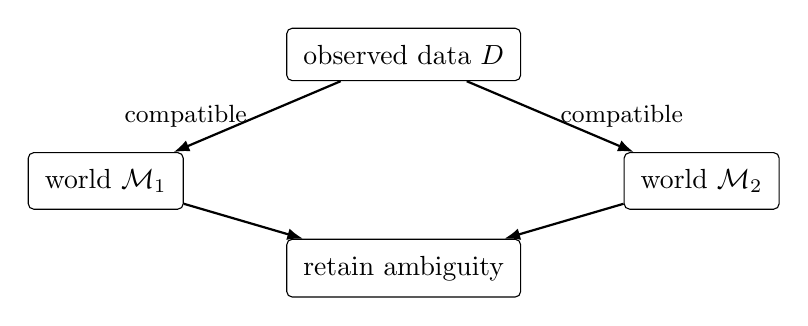
\begin{tikzpicture}[
  node distance=9mm and 13mm,
  box/.style={draw, rounded corners=2pt, inner sep=6pt, align=center},
  arr/.style={-{Latex[length=2mm]}, thick}
]
\node[box] (d) {observed data $D$};
\node[box, below left=of d] (m1) {world $\mathcal{M}_1$};
\node[box, below right=of d] (m2) {world $\mathcal{M}_2$};
\node[box, below=20mm of d] (unc) {retain ambiguity};
\draw[arr] (d) -- node[left, font=\small]{compatible} (m1);
\draw[arr] (d) -- node[right, font=\small]{compatible} (m2);
\draw[arr] (m1) -- (unc);
\draw[arr] (m2) -- (unc);
\end{tikzpicture}
\caption{If two causal worlds are observationally indistinguishable, uncertainty is the correct result.}
\end{figure}

This is not merely a limitation to tolerate. It creates the next question: if two remaining worlds disagree under an intervention, which experiment best separates them?

\section{From passive compatibility to active falsification}

Active Bayesian causal inference already studies how interventions can be selected to reduce uncertainty about causal quantities \cite{toth2022}. AP-002 does not claim the general observe--intervene--update loop as novel.

The eventual extension of the present question is more specific. Suppose uncertainty remains over causal families $K$. For a candidate intervention $a$, each family predicts an interventional outcome distribution

\begin{equation}
p_k(Y\mid\doop(a),D).
\end{equation}

A discriminative experiment would be one on which the families disagree strongly. One possible objective is expected information gain,

\begin{equation}
a^*=\arg\max_a I\!\left(K;Y_a\mid D,\doop(a)\right),
\end{equation}

or a divergence among the family-specific predictive distributions. The conceptual loop is then

\begin{equation}
\boxed{
\text{observe}\rightarrow
\text{maintain possible worlds}\rightarrow
\text{identify uncertainty}\rightarrow
\text{experiment}\rightarrow
\text{falsify/update}
}.
\end{equation}

The scientific value would not be that the system always knows the world. It would be that it can represent when its model class is uncertain and identify evidence capable of resolving some of that uncertainty.

\section{What AP-002 is not}

\begin{itemize}
  \item \textbf{Not an AGI claim.} The immediate objective is robust causal inference under uncertain structural priors. The broader loop resembles a component of scientific reasoning, but it is neither necessary nor sufficient evidence of general intelligence.
  \item \textbf{Not generic OOD detection.} The relevant failure is causal: model families may differ specifically in the intervention quantities they imply, even when ordinary predictive fit is similar.
  \item \textbf{Not ``RAG for causal models.''} The proposal concerns uncertainty over structural assumptions and estimator validity, not retrieval of textual memories.
  \item \textbf{Not a claim that one prior can always be selected.} Ambiguous, overlapping, and unsupported regimes are expected and should be represented explicitly.
  \item \textbf{Not yet a novelty claim.} Prior art exists in active causal inference, Bayesian model averaging, causal PFNs, calibration, causal discovery, and model selection. The exact contribution must be earned experimentally and checked continuously against new literature.
\end{itemize}

\section{Laptop-scale research program}

The first version is intentionally designed so that compute scale cannot become an excuse. Public pretrained models remain frozen. Synthetic data generation and evaluation can run locally.

\subsection*{Experiment 0: reproduce a known result}

Run a released causal PFN on a synthetic treatment-effect problem with known ground truth. Reproduce basic effect estimation and, where practical, a known distribution-shift behavior. If the public model cannot be reproduced reliably, no new claim should be attempted.

\subsection*{Experiment 1: establish complementary causal priors}

Take two frozen models trained under meaningfully different priors, for example a linear-Gaussian family and a richer nonlinear family. Evaluate both across both test families. Let

\begin{equation}
R_{ij}=\mathbb{E}\left[L(F_j(D),\tau)\mid D\sim\Pi_i\right].
\end{equation}

The program is interesting only if there is useful complementarity: the best expert should depend on the regime. If one model dominates across families, adaptive routing adds little.

\subsection*{Experiment 2: infer compatibility using observations only}

Hide the simulator label. Build an intentionally simple compatibility function from observational diagnostics $\phi(D)$:

\begin{equation}
q_k(D)=g_k(\phi(D)).
\end{equation}

The router must never observe true individual treatment effects or counterfactual outcomes. Compare it against the best fixed expert, an unweighted ensemble, simple classical causal estimators, and an oracle router that knows which expert performs best.

\subsection*{Experiment 3: held-out mechanisms and negative controls}

Mechanism families used to design the router are separated from confirmatory families. Examples of held-out variation include threshold effects, Fourier-like mechanisms, heavy-tailed noise, heteroskedasticity, and nonstationarity.

A negative control should deliberately construct two families whose observational distributions are difficult or impossible to distinguish. A scientifically honest compatibility model should become uncertain rather than manufacture separation.

\section{What would count as evidence}

The first useful result is not ``the router classifies worlds accurately.'' The causal objective is downstream reliability.

\begin{table}[h]
\centering
\begin{tabularx}{\textwidth}{>{\bfseries}l X}
\toprule
Quantity & Question \\
\midrule
ATE/CATE error & Does prior-aware selection improve causal-effect estimation? \\
Worst-family risk & Does it reduce catastrophic failure on mismatched worlds? \\
Regret to oracle & How much performance is lost relative to perfect expert selection? \\
Coverage & Are uncertainty intervals honest under prior shift? \\
Router calibration & When compatibility is stated as $70\%$, is that belief empirically meaningful? \\
Abstention quality & Does the system decline to trust unsupported regimes? \\
Held-out transfer & Do gains survive mechanism families never used to design the router? \\
\bottomrule
\end{tabularx}
\caption{Initial evidence criteria.}
\end{table}

The strongest early signal would be a pattern such as

\begin{equation}
R(\text{adaptive}) < R(\text{best fixed})
\end{equation}

on held-out mixtures, accompanied by lower worst-family risk and better-calibrated uncertainty. Average error alone is insufficient.

\section{Kill criteria}

AP-002 should be abandoned or reformulated if any of the following persists after reasonable controls:

\begin{enumerate}
  \item One frozen expert dominates across the relevant prior families, leaving no useful model-selection problem.
  \item Observable data contains too little information to predict which causal expert is safer, so adaptive selection cannot beat a fixed strategy.
  \item A simple fixed ensemble matches the adaptive method on held-out risk and uncertainty.
  \item Apparent routing success disappears when simulator-specific scale, variable order, or other superficial artifacts are controlled.
  \item Gains disappear on held-out mechanism families.
  \item The method becomes confidently decisive in negative-control settings where the candidate worlds are observationally indistinguishable.
\end{enumerate}

A negative result is still useful if it identifies a principled boundary on when prior-family adaptation is possible.

\section{Relationship to broader intelligence}

AP-002 is not designed as an AGI project. Its motivation is narrower and testable. Nevertheless, the problem touches a deeper capability that a scientifically competent intelligent system would plausibly require.

Ordinary inference asks:

\begin{equation}
\text{Given model }M,\text{ what follows?}
\end{equation}

A more reflective system must sometimes ask:

\begin{equation}
\text{Is }M\text{ itself an adequate description of this situation?}
\end{equation}

And, if the answer is uncertain:

\begin{equation}
\text{What evidence would discriminate between the alternatives?}
\end{equation}

This is model criticism rather than merely parameter estimation. In the long run, systems that can expose the failure of their own assumptions, preserve uncertainty, and design tests that distinguish competing explanations would be closer to the logic of scientific inquiry. AP-002 studies a small, falsifiable instance of that capability in causal inference.

\section{Current status}

As of 18 September 2026, AP-002 is an open research problem and experimental program. The immediate next step is not architecture invention. It is reproduction and falsification:

\begin{enumerate}
  \item reproduce released causal-foundation-model behavior locally;
  \item verify that different pretrained causal priors create genuinely complementary experts;
  \item test whether observational compatibility can predict expert reliability;
  \item freeze held-out mechanism families before router tuning;
  \item only then evaluate adaptive prior selection.
\end{enumerate}

No claim of novelty, superiority, or general causal identification is made at this stage.

\begin{thebibliography}{9}

\bibitem{balazadeh2025}
V. Balazadeh, H. Kamkari, V. Thomas, B. Li, J. Ma, J. C. Cresswell, and R. G. Krishnan,
``CausalPFN: Amortized Causal Effect Estimation via In-Context Learning,'' 2025.
\href{https://arxiv.org/abs/2506.07918}{arXiv:2506.07918}.

\bibitem{ma2026}
Y. Ma, D. Frauen, E. Javurek, and S. Feuerriegel,
``Foundation Models for Causal Inference via Prior-Data Fitted Networks,''
\emph{International Conference on Learning Representations (ICLR)}, 2026.
\href{https://proceedings.iclr.cc/paper_files/paper/2026/hash/7f8cabaf2de70e1a9d3eb187f02bd58c-Abstract-Conference.html}{Proceedings}.

\bibitem{li2026}
Z.-R. Li, S.-Y. Liu, T.-Z. Wang, and H.-J. Ye,
``CausalArena: Benchmarking Causal Discovery in the Foundation Model Era,'' 2026.
\href{https://arxiv.org/abs/2609.11897}{arXiv:2609.11897}.

\bibitem{toth2022}
C. Toth, L. Lorch, C. Knoll, A. Krause, F. Pernkopf, R. Peharz, and J. von K\"ugelgen,
``Active Bayesian Causal Inference,''
\emph{Advances in Neural Information Processing Systems}, vol. 35, 2022.
\href{https://papers.nips.cc/paper_files/paper/2022/hash/675e371eeeea99551ce47797ed6ed33e-Abstract-Conference.html}{NeurIPS proceedings}.

\bibitem{pearl2009}
J. Pearl,
\emph{Causality: Models, Reasoning, and Inference}, 2nd ed.
Cambridge University Press, 2009.

\bibitem{peters2017}
J. Peters, D. Janzing, and B. Sch\"olkopf,
\emph{Elements of Causal Inference: Foundations and Learning Algorithms}.
MIT Press, 2017.

\end{thebibliography}

\vfill
\rule{\textwidth}{0.4pt}
{\small\color{muted}
\Austurusa\quad |\quad \href{https://www.austurusa.com}{austurusa.com}\quad |\quad \codeid{AP-002} problem statement v0.1
}

\end{document}
